\documentclass[12pt]{article}

% ——— Standard Packages ———
\usepackage{amsmath,amssymb}
\usepackage{graphicx}
\usepackage[
  top=0.8in,    % instead of the default 1in
  bottom=0.8in,
  left=1in,
  right=1in
]{geometry}
\usepackage{setspace}
\usepackage{cite}
\usepackage[colorlinks=true,linkcolor=blue,citecolor=blue,urlcolor=blue]{hyperref}
\usepackage{appendix}
\usepackage[hang,flushmargin]{footmisc}
\usepackage{caption}
\usepackage{float}
\usepackage{minipage-marginpar}

\captionsetup{font=footnotesize,labelfont=bf}
\renewcommand{\figurename}{Fig.}
% ——— Line Spacing ———
\setstretch{1.5}

% ——— Section Title Formatting ———
\usepackage{titlesec}
\titleformat{\section}
  {\large\bfseries}   % small + bold
  {\thesection}{0.5em}{}    % show number + small gap
\titlespacing*{\section}
  {0pt}{1ex}{0.5ex}         % {left}{space-before}{space-after}
% ——— Subsection formatting ———
\titleformat{\subsection}
  {\normalsize\bfseries}      % normal size + bold
  {\thesubsection}{0.5em}{}   % number + gap
\titlespacing*{\subsection}
  {0pt}{0.75ex}{0.5ex}         % {left}{before}{after}

% ——— Subsubsection formatting ———
\titleformat{\subsubsection}
  {\normalsize\itshape}         % normal size + italic
  {\thesubsubsection}{0.5em}{}  % number + gap
\titlespacing*{\subsubsection}
  {0pt}{0.5ex}{0.25ex}           % {left}{before}{after}

\begin{document}

% ——— All‐in‐One Centered Header ———
\begin{center}
  \large\bfseries
  Quantum Mechanics of the Cooper Pair Box:\\[0.3ex]
  From Charge Qubit to Transmon\\[0.5ex]
\end{center}
\begin{center}
  \normalsize
  Harry Luo\\[0.1ex]
  Physics 531 Final Project, May 2025
\end{center}

% --- Introduction ---
\section{Introduction}
Superconducting circuits containing Josephson junctions provide a platform for building artificial atoms with designable energy spectra, forming the basis of leading quantum computing architectures \cite{Kjaergaard2020}. The Cooper Pair Box (CPB) is a foundational element, governed by the Hamiltonian:
\begin{equation}
\hat{H} = 4 E_C (\hat{N} - n_g)^2 - E_J^{(1)} \cos \hat{\phi} - \frac{E_J^{(2)}}{2} \cos (2 \hat{\phi}),
\label{eq:main_hamiltonian_condensed}
\end{equation}
where $E_C$ is charging energy, $E_J^{(1,2)}$ Josephson energies, $\hat{N}$ number and $\hat{\phi}$ phase operators ($[\hat{\phi}, \hat{N}] = i$), and $n_g$ gate charge. The ratio $E_J/E_C$ controls the tug-of-war between the $E_C$ term (favoring definite $N$, localized charge) and the $E_J$ term (favoring definite $\phi$, localized phase); the uncertainty principle dictates that localization in one variable implies delocalization in the conjugate variable. % <<< MODIFIED: Added hint about uncertainty and conjugate variables >>>
A key challenge is sensitivity to $n_g$ fluctuations (charge noise), causing decoherence. 

This paper explores how the Hamiltonian (Eq.~\eqref{eq:main_hamiltonian_condensed}) in the charging-dominated ($E_C \gg E_J$) and Josephson-dominated ($E_J \gg E_C$) limits lead to different qubit paradigms—the charge qubit and the transmon qubit, respectively—with vastly different sensitivities to this charge noise. We analyze the underlying physical mechanisms and properties, drawing on detailed calculations attached in Appendix~\ref{app:calculations}. 

% --- Charging Regime Section ---
\section{Charging Dominated Regime \& The Charge Qubit}
In this limit ($E_J/E_C \ll 1$), neglecting $E_J$, eigenstates are charge states $|N\rangle$ with energies $E_N^{(0)} = 4E_C(N-n_g)^2$. Because charge $N$ is well-defined, the phase $\phi$ is completely uncertain ($p(\phi)=1/(2\pi)$, Appendix~\ref{app:part_a:subsubsec_i}), a direct consequence of the uncertainty principle. 
The physics becomes interesting near points where adjacent charge states are degenerate, most notably at the charge frustration point $n_g = 1/2$, where $E_0^{(0)} \approx E_1^{(0)}$. Here, standard non-degenerate perturbation theory breaks down because energy denominators vanish, and the effect of the Josephson coupling $E_J^{(1)}$ is strongest, mixing the degenerate states. 
Applying degenerate perturbation theory within the $\{|0\rangle, |1\rangle\}$ subspace yields the effective Hamiltonian (Appendix~\ref{app:part_a:subsubsec_iii}): % <<< MODIFIED: Added "Applying degenerate perturbation theory..." >>>
\begin{equation}
 H_{\text{eff}} \approx \epsilon_0 \hat{\sigma}_z - \frac{E_J^{(1)}}{2} \hat{\sigma}_x, \quad \text{where } \epsilon_0 = 4 E_C (n_g - 1/2).
 \label{eq:main_Heff_charge_condensed}
\end{equation}
The resulting energy levels (Fig.~\ref{fig:main_avoid_crossing_condensed}) show an avoided crossing with minimum gap $E_J^{(1)}$. The linear dependence on $\epsilon_0 \propto (n_g-1/2)$ leads to extreme sensitivity to gate charge fluctuations, as clearly demonstrated by the sharp transition in ground state charge probability (Fig.~\ref{fig:main_charge_prob_condensed}). This charge noise sensitivity is the primary drawback of the charge qubit. Away from degeneracy (e.g., at $n_g=0$), standard perturbation theory shows the leading effect of the Josephson coupling is a small second-order energy shift $E_0^{(2)} \approx -(E_J^{(1)})^2/(8E_C)$ (Appendix~\ref{app:part_a:subsubsec_ii}). % <<< ADDED: Mention of standard PT for E0(2) >>>
\begin{figure}[htbp] 
    \centering
    \begin{minipage}{0.48\textwidth}
        \centering
        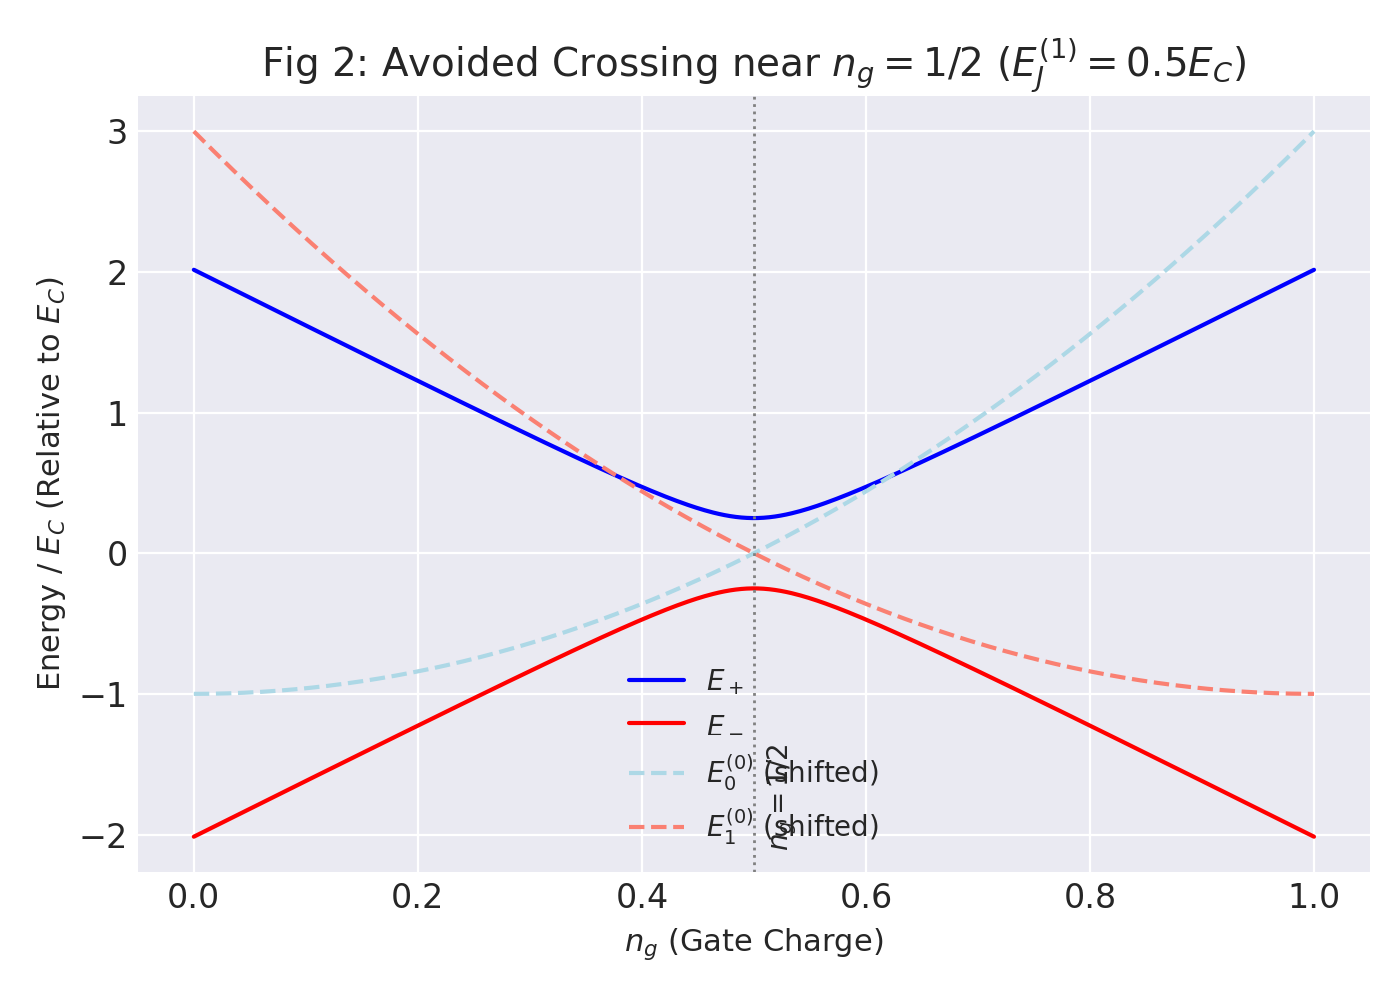
\includegraphics[width=\textwidth]{fig_avoid_crossing.png}
        \caption{Avoided crossing near $n_g = 1/2$ (Charge Qubit). Energy levels vs $n_g$ from $H_{\text{eff}}$ (Eq.~\eqref{eq:main_Heff_charge_condensed}) for $E_J^{(1)} = 0.5 E_C$. Shows linear sensitivity. Appendix~\ref{app:part_a:subsubsec_iii}.}
        \label{fig:main_avoid_crossing_condensed}
    \end{minipage}\hfill 
    \begin{minipage}{0.48\textwidth}
        \centering
        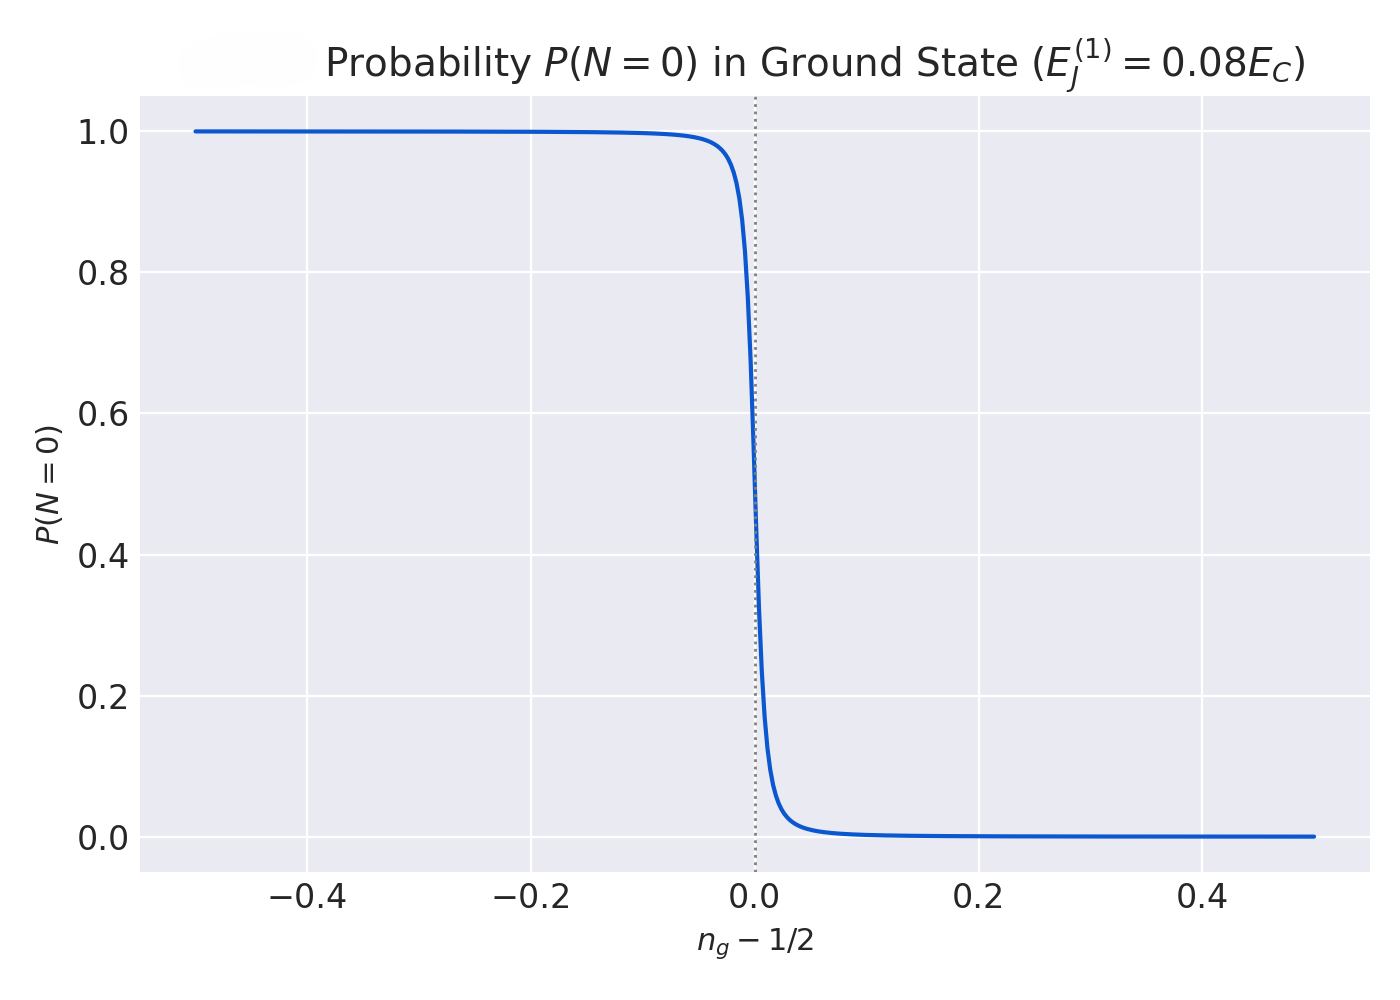
\includegraphics[width=\textwidth]{fig_charge_prob.png}
        \caption{Ground state probability $P(N=0)$ near $n_g=1/2$ for $E_J^{(1)} = 0.08 E_C$. Demonstrates extreme $n_g$ sensitivity. Appendix~\ref{app:part_a:subsubsec_iii}.}
        \label{fig:main_charge_prob_condensed}
    \end{minipage}
\end{figure}

% --- Josephson Regime Section ---
\section{Josephson Dominated Regime \& The Transmon Qubit}
In the opposite limit ($E_J \gg E_C$, with $n_g=0$), the phase $\phi$ localizes near the potential minimum ($\phi=0$). The system approximates an anharmonic oscillator (Appendix~\ref{app:part_b:subsubsec_i}), with the leading behavior captured by the harmonic Hamiltonian:
\begin{equation}
 \hat{H} \approx H_{HO} = V(0) + 4 E_C \hat{N}^2 + \frac{1}{2} k \hat{\phi}^2 ,
 \label{eq:main_H_HO_condensed}
\end{equation}
where $k = E_J^{(1)} + 2 E_J^{(2)}$. Phase localization implies charge delocalization; the ground state charge variance $\Delta N^2 = 1/(2X)$, where $X = \sqrt{8 E_C / k}$, becomes large (Fig.~\ref{fig:main_delta_n_variance_condensed}). This signifies immunity to $n_g$ fluctuations as the state averages over many charge numbers. 

Crucially, the full cosine potential is anharmonic. Treating the subleading $\phi^4$ term as a perturbation to the harmonic oscillator, standard perturbation theory yields corrections to the energy levels characterized by the anharmonicity $\alpha_{anh} = (E_2 - E_1) - (E_1 - E_0)$ (Appendix~\ref{app:part_b:subsubsec_v}): % <<< MODIFIED: Added "standard perturbation theory yields..." >>>
\begin{equation}
 \alpha_{anh} \approx - E_C \frac{E_J^{(1)} + 8 E_J^{(2)}}{E_J^{(1)} + 2 E_J^{(2)}} \approx -E_C .
 \label{eq:main_anharm_condensed}
\end{equation}
This finite $\alpha_{anh}$ (originating from the subleading potential terms) is essential for selectively addressing the $0 \to 1$ qubit transition without driving higher transitions. 

\begin{figure}[htbp] 
    \centering
    \begin{minipage}{0.49\textwidth}
        \centering
        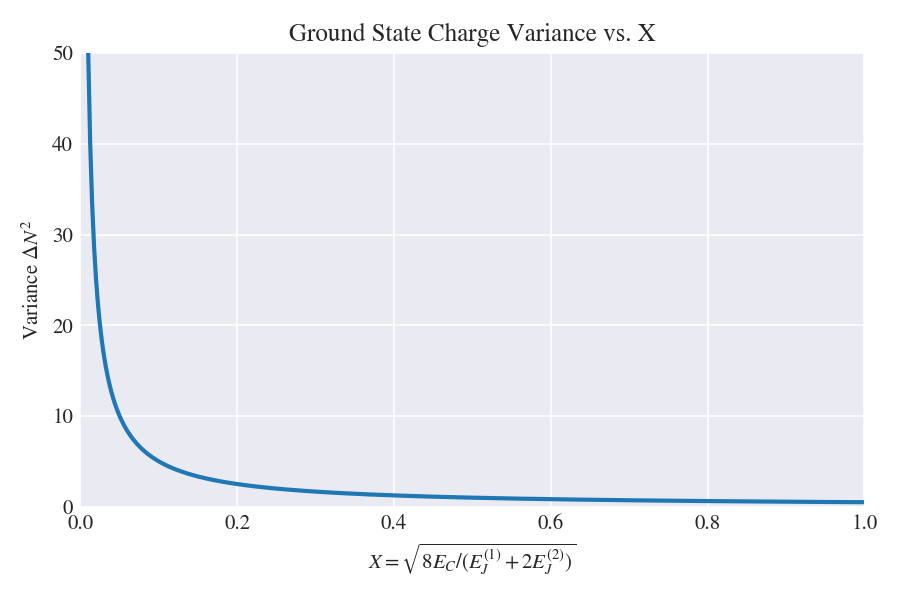
\includegraphics[width=\textwidth]{fig_delta_n_variance.png}
        \caption{Ground state charge variance $\Delta N^2 = 1/(2X)$ vs $X = \sqrt{8 E_C / k}$. Large variance for large $E_J/E_C$ (small $X$) signifies charge delocalization, enabling noise immunity. Appendix~\ref{app:part_b:subsubsec_iii}.}
        \label{fig:main_delta_n_variance_condensed} 
    \end{minipage}\hfill 
    \begin{minipage}{0.49\textwidth}
        \centering
        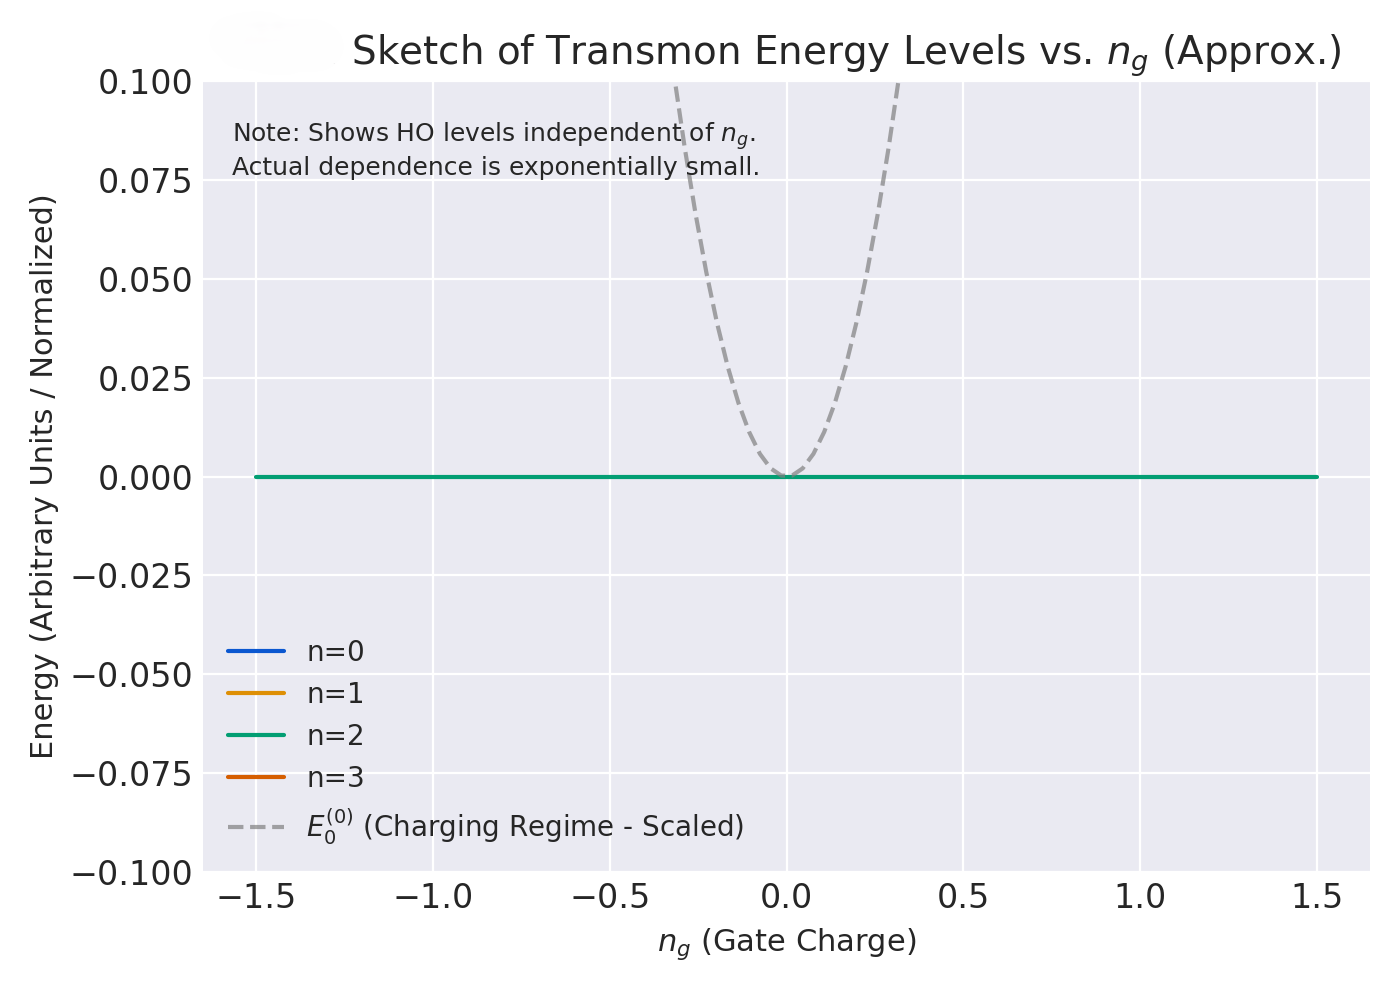
\includegraphics[width=\textwidth]{fig_transmon_levels.png}
        \caption{Conceptual sketch (not to scale): Flat (charge-insensitive) transmon levels ($E_J \gg E_C$, solid) vs parabolic charge qubit levels (dashed $E_0^{(0)}$).} 
        \label{fig:main_transmon_levels_condensed} 
    \end{minipage}
\end{figure}

% --- Interpretation Section ---
\section*{Interpretation: Charge vs. Transmon Synthesis}
The distinct physics in the limiting regimes leads to different qubit designs. The \textbf{charge qubit} ($E_C \gg E_J$) suffers from its linear sensitivity to $n_g$ (Eq.~\eqref{eq:main_Heff_charge_condensed}, Figs.~\ref{fig:main_avoid_crossing_condensed}-\ref{fig:main_charge_prob_condensed}), making it vulnerable to charge noise. 
The \textbf{transmon qubit} ($E_J \gg E_C$) overcomes this by operating with large charge delocalization ($\Delta N^2 \gg 1$, Fig.~\ref{fig:main_delta_n_variance_condensed}). This provides exponential suppression of $n_g$ sensitivity (charge dispersion), making the transmon robust against charge noise—a significant advantage over the charge qubit. 
% <<< CHANGE: Added mention of exactly solvable case >>>
The contrast between these regimes is further illustrated by an exactly solvable case for specific parameters (Appendix~\ref{app:part_c}). The ground state probability density $p(\phi)$ in this model (Fig.~\ref{fig:app_exact_prob}) explicitly shows the evolution from a nearly uniform (charge-like) distribution at low $E_J/E_C$ to one sharply peaked around $\phi=0$ (transmon-like) at high $E_J/E_C$, confirming the transition driven by the energy ratio.



This robustness in the transmon regime must be balanced against the need for sufficient anharmonicity ($\alpha_{anh} \approx -E_C$, Eq.~\eqref{eq:main_anharm_condensed}) for qubit control. Figure~\ref{fig:main_anharm_dispersion_condensed} illustrates this trade-off: increasing $E_J/E_C$ exponentially reduces noise sensitivity (panel b) while the necessary anharmonicity quickly saturates near $-E_C$ (panel a), allowing an optimal operating regime (e.g., $E_J/E_C \sim 50$ \cite{Koch2007, Kjaergaard2020}). The transmon's energy levels become nearly independent of $n_g$, unlike the charge qubit's parabolic dependence (sketched in Fig.~\ref{fig:main_transmon_levels_condensed}).

\begin{figure}[htbp]
  \centering
  \begin{minipage}[t]{0.38\textwidth}
    \centering
    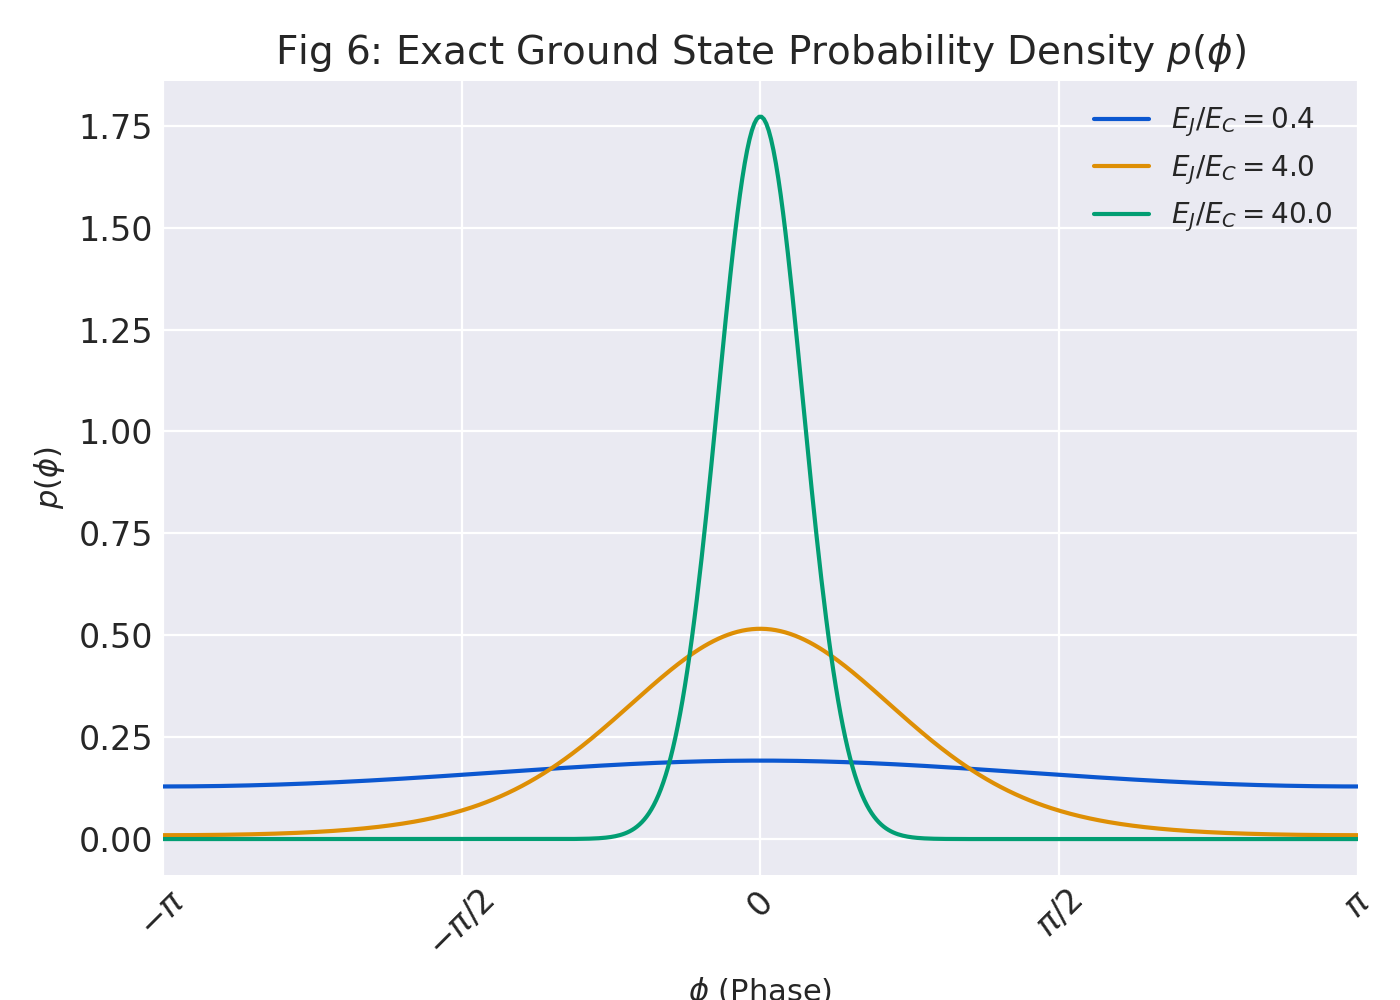
\includegraphics[width=\textwidth]{fig_exact_prob.png}
    \caption{Exact ground state probability density $p(\phi)$ for the special case, plotted for $E_J/E_C = 0.4, 4.0, 40.0$.}
    \label{fig:app_exact_prob}
  \end{minipage}%
  \hfill
  \begin{minipage}[t]{0.6\textwidth}
    \centering
    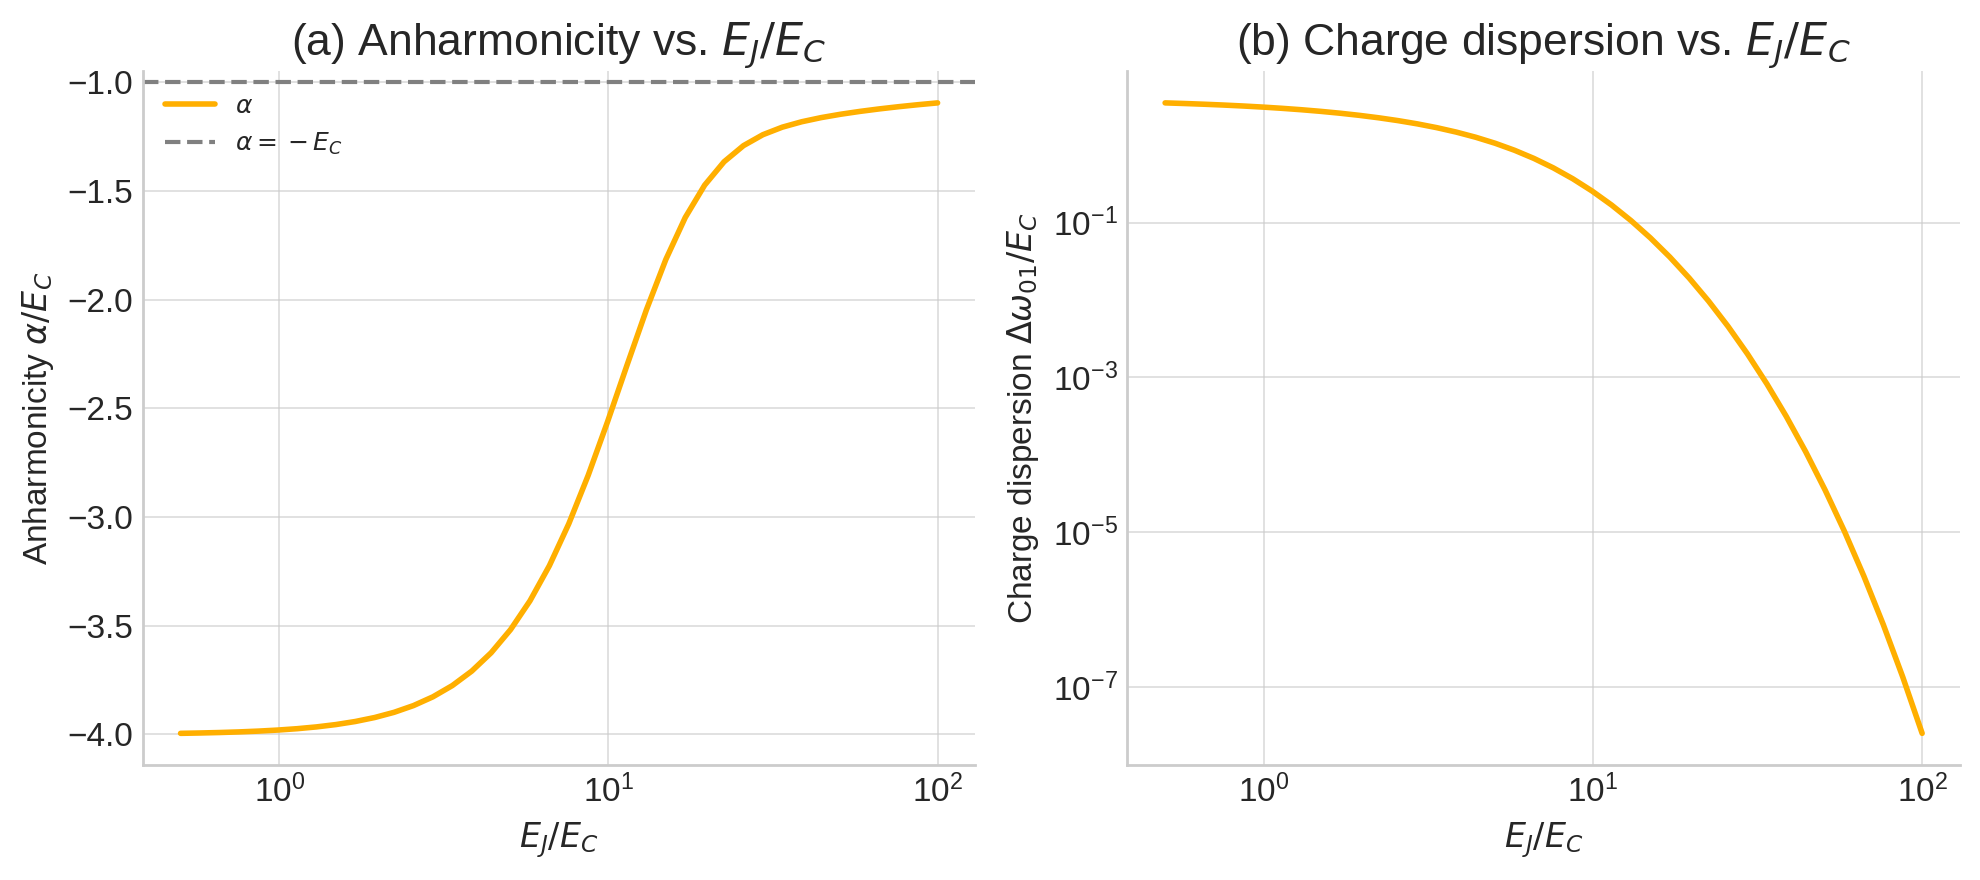
\includegraphics[width=\textwidth]{fig_anharm_dispersion.png}
    \caption{Transmon trade-off vs $E_J/E_C$ (assuming $E_J=E_J^{(1)}, E_J^{(2)}=0$). (a) Anharmonicity $\alpha_{anh}/E_C \to -1$. (b) Charge dispersion $\Delta\omega_{01}/E_C$ decays exponentially \cite{Koch2007}. Appendix~\ref{app:part_b:subsubsec_v}.}
    \label{fig:main_anharm_dispersion_condensed}
  \end{minipage}
\end{figure}



% --- Conclusion ---
\section{Conclusion}
The quantum behavior of the Cooper Pair Box is fundamentally governed by the ratio $E_J/E_C$, dictating a transition between charge-dominated and phase-dominated physics. Our analysis contrasted the two resulting qubit paradigms. In the charge qubit regime ($E_C \gg E_J$), the system exhibits energy levels linearly sensitive to the gate charge $n_g$ near degeneracy points, rendering it highly vulnerable to charge noise, as demonstrated by the sharp dependence of charge occupation probability on $n_g$. % <<< EXPANDED: Explicit summary of charge qubit findings >>>

Conversely, the transmon regime ($E_J \gg E_C$) leverages the dominance of Josephson energy to localize the phase $\phi$, which, by the uncertainty principle, leads to significant delocalization of the charge state $N$. This charge delocalization is the key mechanism providing the transmon with exponential immunity to $n_g$ fluctuations, drastically reducing its susceptibility to charge noise compared to the charge qubit. % <<< EXPANDED: Explicit summary of transmon findings and mechanism >>>
While achieving noise resilience, the transmon retains the essential anharmonicity ($\alpha_{anh} \approx -E_C$) required for qubit addressability. This anharmonicity arises naturally from the higher-order terms of the Josephson cosine potential, ensuring distinct frequencies for qubit transitions. % <<< EXPANDED: Explicit summary of anharmonicity role >>>
This favorable combination of charge noise resilience and sufficient anharmonicity for control explains why the transmon has become a robust and widely implemented superconducting qubit architecture. % <<< EXPANDED: Stronger concluding sentence >>>


% --- Bibliography ---
\begin{thebibliography}{9}
    \bibitem{Koch2007} 
    J. Koch, et al., Phys. Rev. A \textbf{76}, 042319 (2007).
    \bibitem{Kjaergaard2020} 
    M. Kjaergaard, et al., Annu. Rev. Condens. Matter Phys. \textbf{11}, 369–395 (2020).
\end{thebibliography}

\newpage 
% --- Appendix ---
% (Use the concise Appendix version from the previous step)
\begin{appendices}
\section{Appendix: Detailed Calculations}
\label{app:calculations}
Mathematical details supporting the main text results. Units use $\hbar=1$. We generally retain $E_J^{(1)}$ and $E_J^{(2)}$, but note that often $E_J^{(2)}$ is negligible and $E_J$ is used for $E_J^{(1)}$. % <<< CHANGE: Added notation clarification >>>

% --- Appendix Part (a) ---
\subsection[Part (a): Charging Dominated Regime]{Part (a): Charging Dominated Regime ($E_C \gg E_J^{(1)}, E_J^{(2)}$)}
\label{app:part_a}

\subsubsection*{a.i) Eigenstates, Eigenvalues, and Probability Density ($E_J^{(1,2)}=0$)}
\label{app:part_a:subsubsec_i}
Hamiltonian: $\hat{H}_0 = 4 E_C (\hat{N} - n_g)^2$.
Eigenstates: $|N\rangle$ such that $\hat{N}|N\rangle = N|N\rangle, N \in \mathbb{Z}$.
Eigenvalues:
\[ E_N^{(0)}(n_g) = 4 E_C (N - n_g)^2 \]
These levels are plotted in Figure~\ref{fig:app_charge_levels}.
Phase representation wavefunction: $\psi_N(\phi) = \langle \phi | N \rangle = \frac{1}{\sqrt{2\pi}} e^{i N \phi}$.
Probability density: $p_N(\phi) = |\psi_N(\phi)|^2 = 1/(2\pi)$ (uniform).

\begin{figure}[htbp] % <<< CHANGE: Changed [htbp!] to [htbp] for flexibility >>>
    \centering
    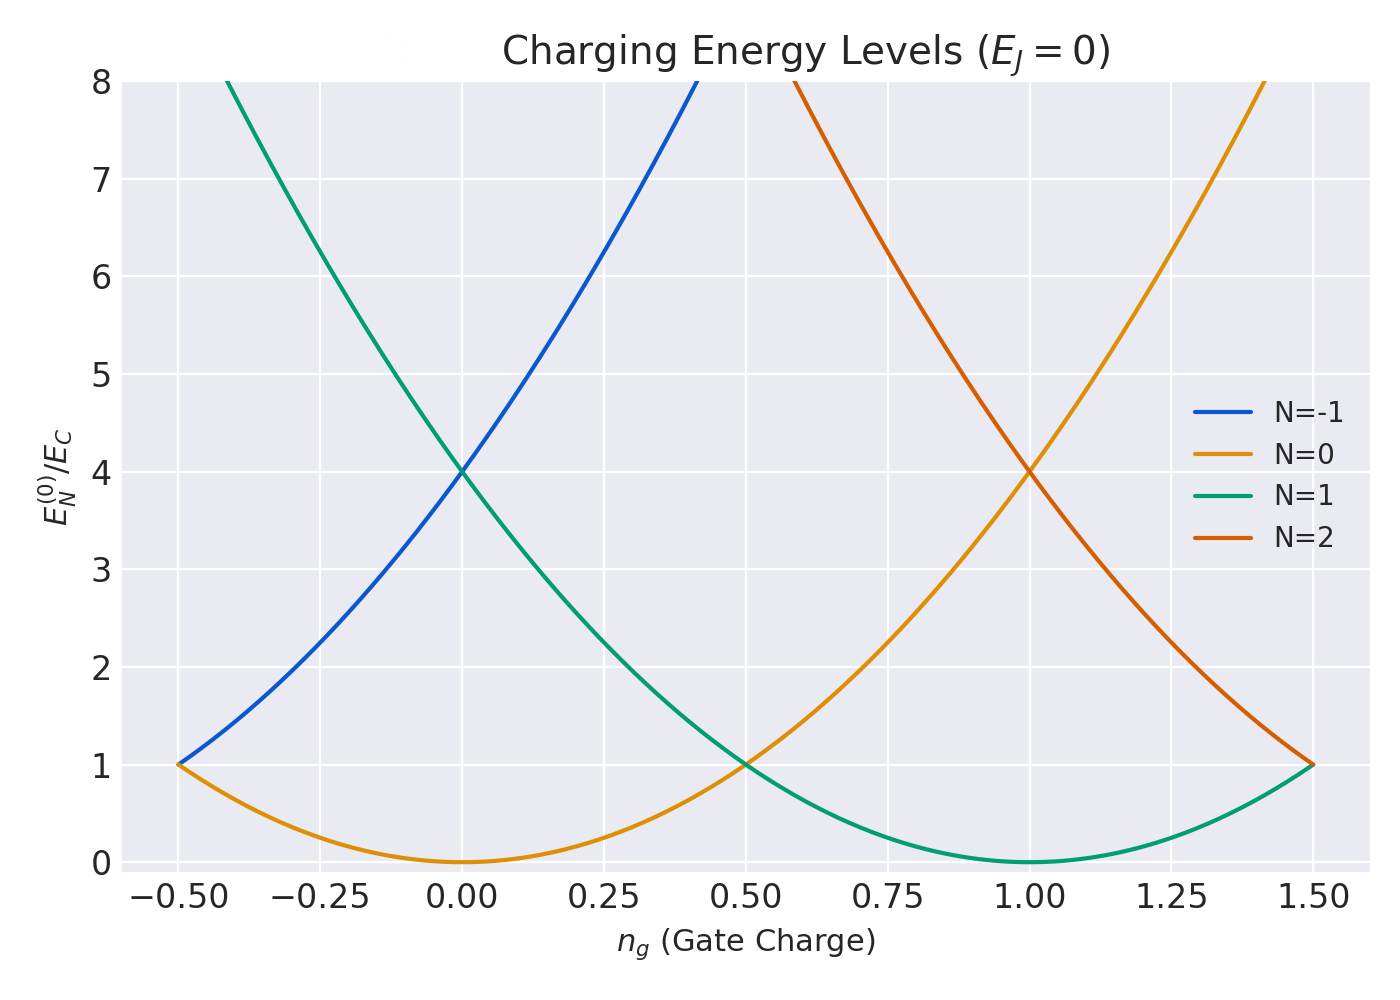
\includegraphics[width=0.6\textwidth]{fig_charge_levels.png}
    \caption{Charging energy levels $E_N^{(0)}/E_C$ vs $n_g$ for $E_J=0$.}
    \label{fig:app_charge_levels} 
\end{figure}

\subsubsection*{a.ii) Perturbation Theory Correction at $n_g=0$}
\label{app:part_a:subsubsec_ii}
Perturbation: $V = -E_J^{(1)} \cos \hat{\phi} - \frac{E_J^{(2)}}{2} \cos (2 \hat{\phi})$.
Unperturbed ground state: $|0\rangle$, $E_0^{(0)}=0$. Valid for $E_J/E_C \ll 1$. % <<< CHANGE: Added domain hint >>>
First-order correction: $E_0^{(1)} = \langle 0 | V | 0 \rangle = 0$.
Second-order correction: $E_0^{(2)} = \sum_{N \neq 0} \frac{|\langle N | V | 0 \rangle|^2}{E_0^{(0)} - E_N^{(0)}}$.
Matrix elements using $\langle N | \cos(k\hat{\phi}) | M \rangle = \frac{1}{2}(\delta_{N, M+k} + \delta_{N, M-k})$:
\[ \langle \pm 1 | V | 0 \rangle = -E_J^{(1)}/2, \quad \langle \pm 2 | V | 0 \rangle = -E_J^{(2)}/4 \]
Energy denominators: $E_0^{(0)} - E_N^{(0)} = -4 E_C N^2$.
Summing contributions ($N=\pm 1, N=\pm 2$):
\[ E_0^{(2)} = 2 \frac{|-E_J^{(1)}/2|^2}{-4 E_C (1)^2} + 2 \frac{|-E_J^{(2)}/4|^2}{-4 E_C (2)^2} = -\frac{(E_J^{(1)})^2}{8 E_C} - \frac{(E_J^{(2)})^2}{128 E_C} \]

\subsubsection*{a.iii) Charge Qubit near $n_g=1/2$}
\label{app:part_a:subsubsec_iii}
Degenerate subspace $\{|0\rangle, |1\rangle\}$ near $n_g=1/2$. Let $n_g = 1/2 + \delta$.
Unperturbed energies: $E_0^{(0)} \approx E_C - 4E_C\delta$, $E_1^{(0)} \approx E_C + 4E_C\delta$.
Perturbation matrix element: $V_{01} = \langle 0 | V | 1 \rangle \approx -E_J^{(1)}/2$.
Hamiltonian matrix (basis $\{|0\rangle, |1\rangle\}$):
\[ H \approx \begin{pmatrix} E_C - 4E_C\delta & -E_J^{(1)}/2 \\ -E_J^{(1)}/2 & E_C + 4E_C\delta \end{pmatrix} \]
Effective Hamiltonian ($H_{\text{eff}} = H - E_C I$, $\epsilon_0 = 4 E_C \delta = 4 E_C (n_g - 1/2)$):
\[ H_{\text{eff}} = \begin{pmatrix} -\epsilon_0 & -E_J^{(1)}/2 \\ -E_J^{(1)}/2 & \epsilon_0 \end{pmatrix} = -\epsilon_0 \hat{\sigma}_z - \frac{E_J^{(1)}}{2} \hat{\sigma}_x \]
Eigenvalues: $E_{\pm} = \pm \sqrt{\epsilon_0^2 + (E_J^{(1)}/2)^2}$.
Ground state ($E_-$) probability in state $|0\rangle$:
\[ P(N=0) = \frac{1}{2} \left( 1 + \frac{\epsilon_0}{\sqrt{\epsilon_0^2 + (E_J^{(1)}/2)^2}} \right) \]
(Sign depends on basis ordering/$\sigma_z$ convention, plot shape is key).

% --- Appendix Part (b) ---
\subsection[Part (b): Josephson Dominated Regime]{Part (b): Josephson Dominated Regime ($E_J^{(1)}, E_J^{(2)} \gg E_C$, $n_g=0$)}
\label{app:part_b}
Valid for $E_J/E_C \gg 1$. % <<< CHANGE: Added domain hint >>>

\subsubsection*{b.i) Harmonic Oscillator Approximation: Levels and Wavefunctions}
\label{app:part_b:subsubsec_i}
Potential $V(\phi) = -E_J^{(1)} \cos \phi - \frac{E_J^{(2)}}{2} \cos (2 \phi)$. Expand around $\phi=0$:
\[ V(\phi) \approx V(0) + \frac{1}{2}V''(0)\phi^2 + \frac{1}{24}V^{(4)}(0)\phi^4 + ... \]
\[ V(0) = -E_J^{(1)} - E_J^{(2)}/2 \]
\[ V''(0) = E_J^{(1)} + 2 E_J^{(2)} \equiv k \]
\[ V^{(4)}(0) = -(E_J^{(1)} + 8 E_J^{(2)}) \]
Approximate Hamiltonian (HO): $\hat{H}_{HO} = V(0) + 4 E_C \hat{N}^2 + \frac{1}{2} k \hat{\phi}^2$.
Effective mass $m^* = 1/(8E_C)$, frequency $\omega = \sqrt{k/m^*} = \sqrt{8 E_C k}$.
Energy levels: $E_n^{(HO)} = V(0) + \omega(n+1/2)$.
Width parameter: $\alpha = (m^* \omega)^{1/4} = (k / (8 E_C))^{1/4}$.
Wavefunctions: $\psi_n^{(HO)}(\phi) = N_n H_n(\alpha \phi) e^{-\alpha^2\phi^2/2}$.

\subsubsection*{b.ii) Probability Density Plot}
\label{app:part_b:subsubsec_ii}
Probability densities $p_n(\phi)=|\psi_n^{(HO)}(\phi)|^2$ for $n=0,1,2$ using $\alpha^2=10$ (for $E_C = (E_J^{(1)}+2E_J^{(2)})/800$) are plotted in Figure~\ref{fig:app_ho_probs}.

\begin{figure}[htbp] % <<< CHANGE: Changed [htbp!] to [htbp] for flexibility >>>
    \centering
    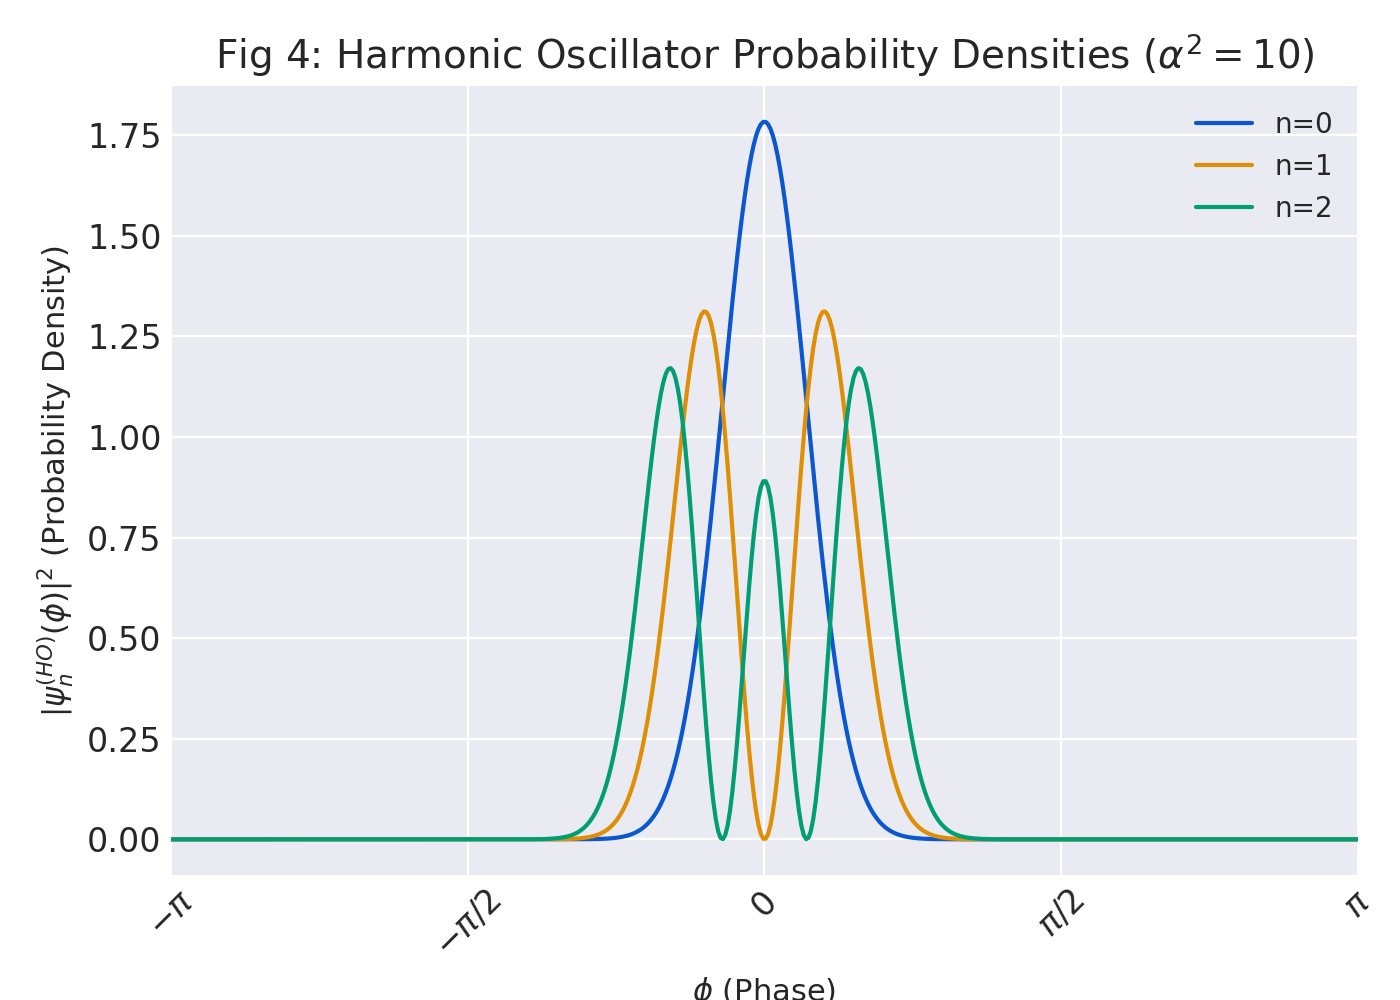
\includegraphics[width=0.6\textwidth]{fig_ho_prob.png} 
    \caption{Approximate HO probability densities $p_n(\phi)$ for $n=0,1,2$ with $\alpha^2=10$.}
    \label{fig:app_ho_probs} 
\end{figure}

\subsubsection*{b.iii) Charge Expectation Value and Variance}
\label{app:part_b:subsubsec_iii}
Ground state average: $\langle \hat{N} \rangle_0 = 0$.
Variance: $\Delta N^2 = \langle \hat{N}^2 \rangle_0$.
Relation to kinetic energy: $\langle KE \rangle_0 = 4 E_C \langle \hat{N}^2 \rangle_0 = \omega/4$.
\[ \langle \hat{N}^2 \rangle_0 = \frac{\omega}{16 E_C} \]
Using $X = \sqrt{8 E_C / k}$: $\omega = \sqrt{8 E_C k} = \sqrt{8 E_C (8E_C/X^2)} = 8E_C/X$.
\[ \Delta N^2 = \frac{8E_C/X}{16 E_C} = \frac{1}{2X} \]

\subsubsection*{b.iv) Subleading Correction to Energy Levels}
\label{app:part_b:subsubsec_iv}
Perturbation: $V_{pert} = \frac{1}{24}V^{(4)}(0) \hat{\phi}^4 = -\frac{E_J^{(1)} + 8 E_J^{(2)}}{24} \hat{\phi}^4$.
First-order correction: $E_n^{(1)} = \langle n | V_{pert} | n \rangle$.
Expectation value: $\langle n | \hat{\phi}^4 | n \rangle = (\frac{4E_C}{\omega})^2 (6n^2 + 6n + 3)$.
\[ E_n^{(1)} = -\frac{E_J^{(1)} + 8 E_J^{(2)}}{24} \left(\frac{4E_C}{\omega}\right)^2 (6n^2 + 6n + 3) \]
Substituting $\omega^2 = 8 E_C (E_J^{(1)} + 2 E_J^{(2)})$:
\[ E_n^{(1)} = -\frac{E_C (E_J^{(1)} + 8 E_J^{(2)})}{12 (E_J^{(1)} + 2 E_J^{(2)})} (6n^2 + 6n + 3) \equiv - C (6n^2 + 6n + 3) \]
Corrections: $E_0^{(1)} = -3C$, $E_1^{(1)} = -15C$, $E_2^{(1)} = -39C$.

\subsubsection*{b.v) Interpretation: Are Levels Equidistant?}
\label{app:part_b:subsubsec_v}
Energy differences:
\[ E_1 - E_0 \approx \omega - 12C \]
\[ E_2 - E_1 \approx \omega - 24C \]
Anharmonicity:
\[ \alpha_{anh} = (E_2 - E_1) - (E_1 - E_0) \approx -12C = - E_C \frac{E_J^{(1)} + 8 E_J^{(2)}}{E_J^{(1)} + 2 E_J^{(2)}} \]
Since $\alpha_{anh} \neq 0$, levels are not equidistant. If $E_J^{(2)}=0$, $\alpha_{anh} = -E_C$.

% --- Appendix Part (c) ---
\subsection[Part (c): Exactly Solvable Case]{Part (c): Exactly Solvable Case ($E_J^{(1)}=E_J, E_J^{(2)}=E_J^2/(4E_C)$)}
\label{app:part_c}
Parameters: $n_g = 0$, $E_J^{(1)}=E_J$, $E_J^{(2)}=E_J^2/(4E_C)$.

Hamiltonian: \[\hat{H} = 4E_C \hat{N}^2 - E_J \cos(\hat{\phi}) - \frac{E_J^2}{8E_C} \cos(2\hat{\phi}).\]
Exact ground state energy: $E_0 = -E_J^2 / (8 E_C).$
Unnormalized ground state wavefunction: $\psi_0(\phi) = A \exp(\frac{E_J}{4 E_C} \cos \phi)$.
Normalization integral: \[\int_{-\pi}^{\pi} |\psi_0(\phi)|^2 d\phi = 2\pi |A|^2 I_0(E_J / (2 E_C)),\] where $I_0$ is the modified Bessel function of the first kind.
Normalized probability density:
\[ p(\phi) = \frac{\exp(\frac{E_J}{2 E_C} \cos \phi)}{2 \pi I_0(E_J / (2 E_C))} \]
This is plotted in Figure~\ref{fig:app_exact_prob}.
Comparison: $E_0$ matches $E_0^{(2)}$ from Sec.~\ref{app:part_a:subsubsec_ii} if $E_J^{(1)}=E_J, E_J^{(2)}=0$.



\end{appendices}

\end{document}
